\hypertarget{P162}{}
\begin{solution}{normal} % 162
An electron with velocity $v$ moves in a homogeneous magnetic field $\textbf{\textit{B}}$, where $\textbf{\textit{v}}\bot \textbf{\textit{B}}$. Determine the radius of the electron's trajectory.
\end{solution}

\hypertarget{P163}{}
\begin{solution}{normal} % 163
A beam of electrons is emitted from a point source. The magnitudes of the velocities $v$ of the electrons are equal, but they are scattered by an angle of up to $\alpha$ with respect to the direction of the homogeneous magnetic field $B$ in the space, where $\alpha\ll 1$. At what distance from the point source does the electron beam focus again?
\end{solution}

\hypertarget{P164}{}
\begin{solution}{normal} % 164
Two parallel electrodes (a cathode and an anode) are located a distance $d$ from each other in a vacuum. A positive potential $U$ is applied from the cathode to the anode. From the surface of the cathode, an electron with initial velocity zero is accelerated by the electric field. How strong of a magnetic field $\textbf{\textit{B}}$ perpendicular to the electric field must be generated between the electrodes so that the electron no longer reaches the anode?
\end{solution}

\hypertarget{P165}{}
\begin{solution}{normal} % 165
Two coaxial cylindrical conductors are located in a vacuum. The inner (cathode) radius is $a$ and the outer (anode) radius is $b$. The anode is given a positive potential $U$ with respect to the cathode. There is a homogeneous magnetic field $\textbf{\textit{B}}$ in the space between the cylinders. An electron begins to move with initial speed zero from the surface of the cathode due to the electric field. Determine the critical value of $\textbf{\textit{B}}$ for which the electron no longer reaches the anode.
\end{solution}

\hypertarget{P166}{}
\begin{solution}{normal} % 166
An electron with initial velocity $v_0$ travels in a homogeneous electric and magnetic field. The vectors $v_0,\textbf{\textit{E}}$, and $\textbf{\textit{B}}$ are all perpendicular to each other and $v_0=\textbf{\textit{B}}\times\textbf{\textit{E}}$. What is the trajectory of the electron? What is its average speed $\left<v\right>$? Assume that $E/B\ll c$ and $v\ll c$.
\end{solution}

\hypertarget{P167}{}
\begin{solution}{normal} % 167
In metals, each atom donates, on average, one valence electron. Determine the drift velocity of electrons in copper wire with current density $5\;\text{A}/\text{mm}^2$. The density of copper is $8900\;\text{kg}/\text{m}^3$ and its molar mass is $63.5\;\text{g}/\text{mol}$.
\end{solution}

\hypertarget{P168}{}
\begin{solution}{normal} % 168
Two identical metal spheres of radius $r$ are placed in a homogeneous conductive medium with resistivity $\rho$. The distance between the spheres is much larger than their radius. What is the resistance between the spheres?
\end{solution}

\hypertarget{P169}{}
\begin{solution}{normal} % 169
One problem in determining the resistivity $\rho$ of a semiconductor is the unknown voltage drop across the contacts. This problem can be solved with the following method, which we analyze here using a semi-infinite thin plate (with thickness $h$) for simplicity. Let the four contacts be soldered to the edge of the plate as shown in the diagram below. a) Current I passes though contacts $A$ and $B$. Show that a voltmeter connected between contacts $C$ and $D$ measures a voltage of
$$U=\dfrac{I\rho}{\pi h}\ln\left(\dfrac{(a+b+c)b}{(a+b)(b+c)}\right).$$
Let the ratio $U/I$ be $R_{AB,CD}$. b) Show analogously that when current $I$ passes through contacts $B$ and $C$, then
$$R_{BC,AD}=\dfrac{\rho}{\pi h}\ln\left(\dfrac{(a+b)}{(b+c)}{ac}\right)$$
c) Show that
$$\exp(\pi hR_{AB,CD}/\rho)+\exp(\pi hR_{BC,AD}/\rho)=1$$
The obtained relationship allows us to determine $\rho$ after measuring $R_{AB,CD}$ and $R_{BC,AD}$.
\begin{center}
    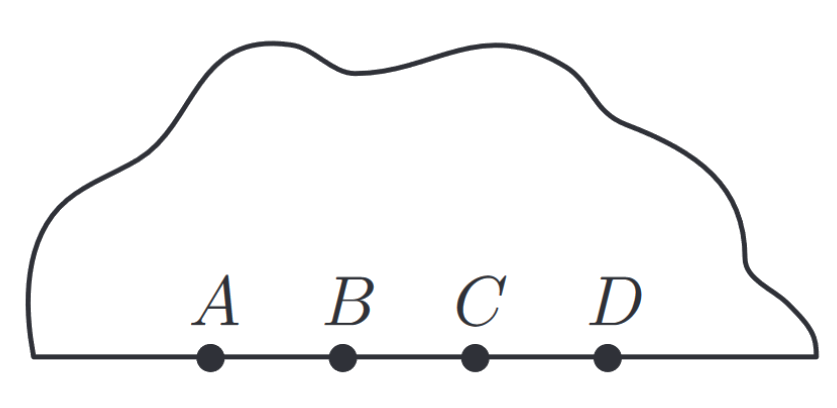
\includegraphics[width=0.4\textwidth]{S7 Figures/S7-169.png}
\end{center}
\blfootnote{It is not specified what $a$, $b$, and $c$ are, but it is likely that $a=AB$, $b=BC$, and $c=CD$}
\end{solution}

\hypertarget{P170}{}
\begin{solution}{normal} % 170
With the method described below, it is possible to measure the resistivity of a material without attaching contacts to the material. A disk-shaped piece of material is placed in a homogeneous magnetic field generated inside a solenoid so that the axis of the disk is parallel to the axis of the solenoid. The solenoid is supplied by an AC source with frequency $\omega$ such that $B(t)=B_0\cos(\omega t)$. The disk has radius $R$ and thickness $d$. Determine the resistivity of the disk if the disk dissipates power $P$. \textit{Note:} You may need the formula $\left<\sin^2\alpha\right>=\left<\cos^2\alpha\right>=1/2$ and the integral $\int x^ndx=x^{n+1}/(n+1)$.
\end{solution}

\hypertarget{P171}{}
\begin{solution}{normal} % 171
A metal plate is located in a homogeneous magnetic field $\textbf{\textit{B}}$ that is perpendicular to the surface of the plate. Determine the drag force caused by the eddy currents in the plate as the plate moves at a speed $\textbf{\textit{v}}$ perpendicular to $\textbf{\textit{B}}$. The area of the plate is $S$, its thickness is $d$, and it has resistivity $\rho$. \textit{Note:} There are several ways to get an approximate answer. One possibility is to use conservation of energy by estimating the heat generated in the plate due to the eddy currents.
\end{solution}
\newpage
\hypertarget{P172}{}
\begin{solution}{normal} % 172
Determine the strength of the transverse electric field due to the Hall effect for the situation shown in the image below. Assume that there is only one type of charge carrier in the material, with charge $q$ and charge carrier density $n$.
\begin{center}
    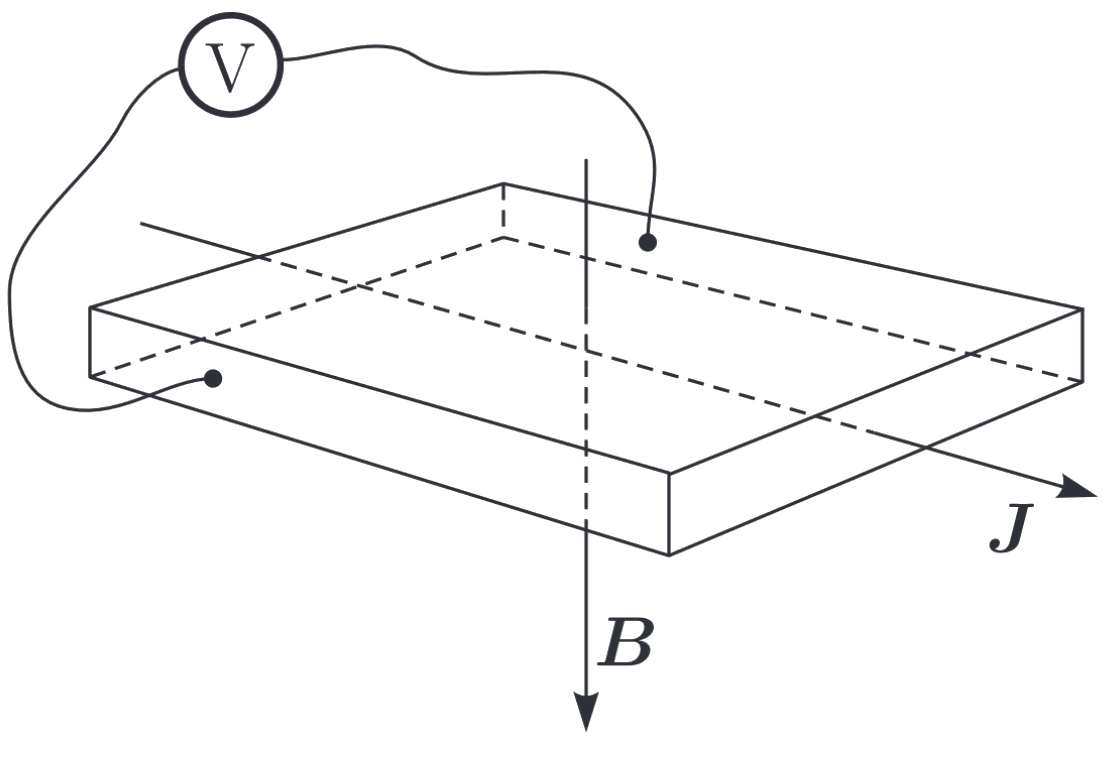
\includegraphics[width=0.5\textwidth]{S7 Figures/S7-172.png}
\end{center}
\end{solution}

\hypertarget{P173}{}
\begin{solution}{normal} % 173
A semiconductor that measures the strength of a magnetic field using the Hall effect is called a Hall sensor. Construct a circuit diagram for a wattmeter if a Hall sensor, solenoid, and voltmeter are used.
\end{solution}

\hypertarget{P174}{}
\begin{solution}{normal} % 174
An electromagnetic pump can be used to pump liquids with good electrical conductivity (a schematic is shown in the figure below). A liquid with resistivity $\rho$ moves at speed $v$ through the pump. The vectors $\textbf{\textit{v}},\textbf{\textit{B}}$, and $\textbf{\textit{E}}$ are all mutually perpendicular. a) Show that the fluid is subjected to a force $\textbf{\textit{F}}=B^2(\textbf{\textit{u}}-\textbf{\textit{v}})/\rho$, where $\textbf{\textit{u}}=\textbf{\textit{E}}\times\textbf{\textit{B}}/B^2$. b) Show that the maximum efficiency of the pump is $0.5$. Assume that the magnetic field creates a permanent magnet and that edge effects are negligible. 
\begin{center}
    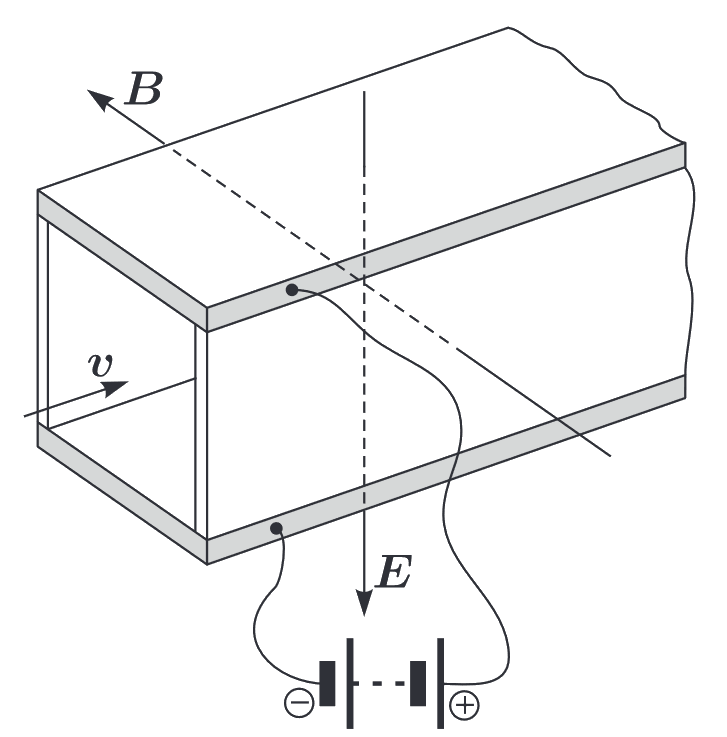
\includegraphics[width=0.5\textwidth]{S7 Figures/S7-174.png}
\end{center}
\end{solution}

\hypertarget{P175}{}
\begin{solution}{normal} % 175
A homopolar motor consists of a copper disk attached to a shaft that rotates in a homogeneous magnetic field $\textbf{\textit{B}}$ directed parallel to the axis of the disk. Current flows into the disk through the shaft and exits through the side of the disk. The radius of the shaft is $a$, the radius of the disk $b$, and the thickness of the disk $h$. The resistivity of the disk is $\rho$. a) Determine the torque $M$ exerted on the disk by the magnetic field when a current $I$ flows through it. b) Determine the heat $P$ dissipated by the disk when a current $I$ flows through it. c) Find the potential difference $U$ between the axis and the edge of the disk when it is rotating at an angular velocity $\omega$. d) Show that conservation of energy holds in the form $VI=M\omega+P$. \textit{Note:} The problems requires taking a few simple integrals: $\int xdx=x^2/2,\int (1/x)dx=\ln x$.
\end{solution}